\RequirePackage[ngerman=ngerman-x-latest]{hyphsubst}
\documentclass[ngerman]{tudscrreprt}

%\usepackage{selinput}
\usepackage[utf8]{inputenc}
\usepackage[ngerman]{babel}
\usepackage[T1]{fontenc}
\usepackage{scrhack}
\usepackage{tudscrsupervisor}
\usepackage{color}
\usepackage{transparent}
\usepackage{url}
\usepackage{graphicx,subfig}
\graphicspath{{img/}}
\usepackage{wrapfig}
\usepackage{csquotes}
\usepackage{amsmath}
\usepackage{amsfonts}
\usepackage{amssymb}
\usepackage{makeidx}
\usepackage{mcode}
\usepackage{float}
\usepackage{trfsigns}
%\usepackage[backend=biber,style=alphabetic]{biblatex}

% Literaturverzeichnis
%\addbibresource{bibHauptseminar.bib}

\usepackage[linkcolor=black]{hyperref}

\renewcommand\thesection{\arabic{section}}
\renewcommand\thesubsection{\thesection.\arabic{subsection}}

\begin{document}
\faculty{Fakultät Elektrotechnik und Informationstechnik}
\institute{Institut für Nachrichtentechnik}
\chair{Deutsche Telekom Professur für Kommunikationsnetze}
\date{13.07.2016}
\title{Compressed Compute-and-Forward mit korrelierten Audiosignalen}

\author{%
	Lucas Weber
	\matriculationnumber{3969535}
	\dateofbirth{10.01.1995}
	\and%
	Raphael Hildebrand
	\matriculationnumber{3948419}
	\dateofbirth{24.05.1995}
	\and%
	Florian Roth
	\matriculationnumber{3966248}
	\dateofbirth{13.01.1994}
	\and%
	Orell Garten
	\matriculationnumber{3948375}
	\dateofbirth{09.07.1993}
}
\matriculationyear{2013}
\supervisor{Dipl.-Ing. Carsten Hermann}
\professor{Prof. Dr.-Ing. Dr. h.c. Frank H. P. Fitzek}

\maketitle
 
% \TUDoption{abstract}{multiple,section}
% \begin{abstract}
%  Dies ist der deutschsprachige Teil der Zusammenfassung, in dem die
%  Motivation sowie der Inhalt der nachfolgenden wissenschaftlichen
%  Abhandlung kurz dargestellt werden.
% \nextabstract[english]
%  This is the english part of the summary, in which the motivation and
%  the content of the following academic treatise are briefly presented.
% \end{abstract} 
 
\confirmation

\tableofcontents
\newpage

\section{Aufgabenstellung}
Es ist ein Programm zu entwerfen, welches Audiodateien einliest und dateiweise die beiden Stereo-Kanäle miteinander korreliert. Es sollen Maßzahlen entworfen und berechnet werden, die wesentliche charakteristische Eigenschaften der Korrelationsfunktion, insbesondere den Anteil dominanter Komponenten und deren Abklingverhalten, widerspiegeln. Dafür sind Audiosignale aufzunehmen, bezüglich der verwendeten Maße zu klassifizieren und entsprechend ihrer Klassifzierung systematisch abzuspeichern.
%%%%%%%%%%%%%%%%%%%%%%%%%%%%%%
\section{Motivation}
Im Jahr 2022 werden 500 Milliarden internetfähige Geräte erwartet, die mit einander kommunizieren sollen. Das führt zu extrem hohen Datenmengen, die in kürzestmöglicher Zeit von A nach B transportiert werden müssen. Große Herausforderungen bestehen darin, dass man sehr kurze Verzögerungszeiten und eine hohe Widerstandsfähigkeit garantieren muss. Idealerweise benötigen die Geräte wenig Energie. Ein Ansatz zur Lösung dieses Problems ist die Netzwerkcodierung.\newline
In bestimmten Szenarien ist eine große Anzahl an Geräten mit Sensorik zu Erfassung der Umgebung mit hohen Anforderungen an die Netzwerkkapazität zur Übertragung der erfassten Daten verbunden. Es stellt sich die Frage, wie viele Sensoren für eine ausreichend genaue Abbildung benötigt werden. Da die Quellen teilweise korrelierte Datenströme erzeugen, lässt sich die zu übertragende Gesamtdatenmenge reduzieren, was durch eine geeignete Kombination von Netzwerkcodierung mit Methoden des Compressed Sensing erreicht werden soll.

%%%%%%%%%%%%%%%%%%%%%%%%%%%%%%
\section{Theoretische Vorbetrachtung}
\subsection{Korrelationsfunktion}
\subsection{Parameter}
\subsection{Gauß-Regression}

%%%%%%%%%%%%%%%%%%%%%%%%%%%%%%
\section{Verfügbare Technik}
\subsection{Software}
Softwareseitig haben wir Octave benutzt. Als freie Alternative zu Matlab vereint Octave gute Performance, syntaktische Gleichheit zu Matlab, sowie kostenfreie Benutzung unter einem Dach. Im Vergleich mit Python haben wir festgestellt, dass die Geschwindigkeit aufwendiger Rechnungen, wie der Korrelation, bei Python schlechter ist. Somit haben wir uns für Ocatve entschieden. Um unseres selbstgeschriebenes Programm zu verifizieren haben wir eine Autokorrelation durchgeführt und diese mit der von Audactity berechneten AKF verglichen. Wir sind dabei zu dem Ergebnis gekommen, dass unser Programm funktioniert.
\subsection{Hardware}
Uns standen zwei hochwertige Kondensatormikrofone (M5 Matched Pair Compac 1/2" Cardioid Condenser Microphones von Rode zur Verfügung. Diese Mikrofone sind für dieses Projekt besonders geeignet, da durch die Abstimmung (matched pair) nur die Unterschiede im Signale vor der Aufnahme Einfluss auf die Korrelation haben. Für die Digitalisierung der Signale stand uns ein hochwertiges Audio-USB-Interface zur Verfügung ( Scarlett 2i2 von Focusrite) zur Verfügung. Die Aufnahmen wurden in .wav gespeichert und sind somit verlustfrei. Außerdem konnten wir ein Stativ mit einer Mikrofonschiene verwenden, wodurch die Mikrofone konstanten Abstand hatten. Zur Erzeugung eines reproduzierbaren Klangsignales wurde eine portable Bluetooth-Anlage (Soundlink III von Bose) verwendet.
%%%%%%%%%%%%%%%%%%%%%%%%%%%%%%
\section{Programm}
\subsection{Aufbau des Programms}
Das Programm ist in 3 große Teile gegliedert. Dazu zählt das Einlesen der Audiodateien, die benötigte Signalverarbeitung inklusiver Berechnung der gewünschten Parameter und das Speichern der gewonnenen Werte in Form einer Excel-Datei.
\paragraph{Einlesen der Audiodaten}
Die Audiodateien liegen im WAV-Format als Stereoaufnahme vor. Zunächst wird eine Liste mit allen Dateien in einem bestimmten Ordner erstellt, damit die Dateien nacheinander eingelesen werden können. Im nächsten Schritt werden die beiden Kanäle voneinander getrennt, um diese dann in die Signalverarbeitung zu übergeben.
\paragraph{Signalverarbeitung}
Das Kernstück der Signalverarbeitung ist eine periodische Korrelationsfunktion, die den linken und rechten Kanal miteinander korreliert. Die dabei entstandene Korrelationsfunktion wird dann weiter untersucht. Als nächstes wird eine Art Einhüllende berechnet, die ein Maß für die Steilheit der Kurve ist. Wie bereits im Abschnitt "Gauß-Regression" beschrieben, wird dann mit Hilfe der Methode der kleinsten Quadrate eine Gauß-Glocke so angepasst, dass sie den Verlauf der Hüllkurve der KKF möglichst gut abbildet. Die Parameter ripple, $\sigma$, Gleichanteil und Zeitverschiebung des Maximums aus dem Ursprung werden danach an eine Funktion übergeben, die diese Daten in einer Excel-Tabelle speichert.
\paragraph{Speicherung}
Die Speicherung der Daten erfolgt in einer Excel-Datei. Dabei wird zu erst der Dateiname des Samples und alles dazugehörigen Werte gespeichert. Außerdem wird noch ein Link zum Graphen der Korrelationsfunktion angegeben, damit man sich diese bei der Auswahl der Test-Signale anschauen kann.

\subsubsection{Programmablaufplan}
\begin{figure}[ht!]
\centering
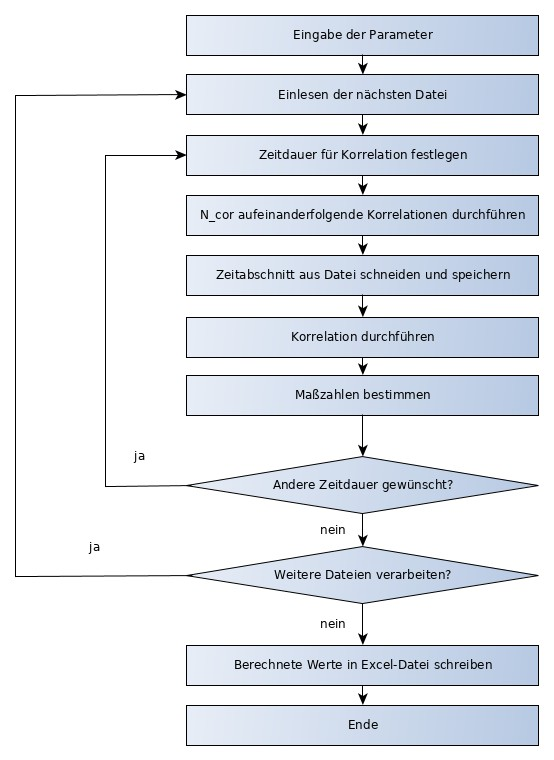
\includegraphics[scale=0.6]{img/pap}
\caption{Programmablaufplan}
\label{figure1}
\end{figure}

\subsection{Mögliche Einstellungen}
Im Code gibt es diverse Eintellungen, die das Verhalten des Programms je nach Wunsch des Anwenders verändern. Diese sind am Beginn der main.m-Datei festgelegt und werden im folgenden beschrieben:
\begin{itemize} 
\item $path$ - Pfad zur Sammlung der WAV-Dateien
\item $excel\_path$ - Pfad unter dem Excel-Datei mit Lösungen gespeichert wird
\item $output$ - Unterscheidung, ob Ergebnisse gespeichert oder angezeigt werden
\item $calc$ - Wechsel zwischen Berechnung im Zeit- und Frequenzbereich möglich.
\item $x\_axes$ - Unterscheidung, ob Korrelation gegen Samples oder Zeit aufgetragen wird
\item $priority$ - Unterscheidung, ob angegebene Blocklänge oder Zeitdauer priorisiert wird
\item $t\_start$ - Startzeitpunkt der Korrelation
\item $t\_dur$ - Array $A1$ mit Menge an Zeitdauern die korrelierten werden sollen, Korrelation beginnt immer bei $t\_start$
\item $Ncor\_init$ - Array, mit identischer Länge zu $A1$. Gibt an wie oft korrespondierender Eintrag in $A1$ hintereinander korreliert wird. 
\item $Lcor$ - Blocklänge der Korrelation
\end{itemize}
\subsection{Probleme} 


%%%%%%%%%%%%%%%%%%%%%%%%%%%%%%
\section{Signalauswahl}
Wir haben für die Aufnahme der Signale viel verschiedene Situationen ausgesucht, um ein möglichst breites Spektrum an Raum-Effekten zu erhalten. Aufnahmeorte waren beispielsweise der Platz vor dem HSZ, die Wiese zwischen Physik- und Mathematikgebäude, sowie der Trefftzbau. Außerdem wurde in einer Wohnung gemessen, um Effekte von schallabsorbierenden Stoffen wie Teppich oder Bett zu erhalten. Soweit mgölich, haben wir die natürliche Geräuschkulisse am jeweiligen Ort eingefangen. Zusätzlich dazu wurde ein definiertes Signal mittels eines Lautsprechers erzeugt, um Direktschall zu nutzen. Bei diesen Aufnahmen sollten die Effekte des Raumes am deutlichsten hervortreten.
\subsection{Beispielsignal}
\subsection{Probleme bei der Signalauswahl}

\section{Zusammenfassung}

\newpage
\begin{thebibliography}{}
\bibitem[ISV]{bezug1} R"udiger Hoffmann, Matthias Wolff: Intelligente Signalverarbeitung 1. Springer Verlag Berlin Heidelberg 2014
\bibitem[NT]{bezug2} Prof. Dr.-Ing. Dr. h.c. Gerhard P. Fettweis: Einf"uhrung in die Nachrichtentechnik. Technische Universit"at Dresden, Fakult"at Elektrotechnik, Vodafone Stiftungslehrstuhl Mobile Nachrichtensysteme, D-01062 Dresden Sommersemester 2015
\bibitem[KN]{bezug} Prof. Dr.-Ing. Dr. h.c. Frank H. P. Fitzek: Vorlesung Kooperative Kommunikationssysteme, Dresden 3.6.2016, https://bildungsportal.sachsen.de/opal/auth/RepositoryEntry/11031117850/\\CourseNode/93439736179888/dirpath/Lectures/CoopCom-Lecture10-03062016.pdf, downloaded: 12.07.2016
\end{thebibliography}

\end{document}
